\ifx\allfiles\undefined
\documentclass[12pt, a4paper, oneside, UTF8]{ctexbook}
\def\path{../config}
\usepackage{amsmath}
\usepackage{amsthm}
\usepackage{amssymb}
\usepackage{array}
\usepackage{xcolor}
\usepackage{graphicx}
\usepackage{mathrsfs}
\usepackage{enumitem}
\usepackage{geometry}
\usepackage[colorlinks, linkcolor=black]{hyperref}
\usepackage{stackengine}
\usepackage{yhmath}
\usepackage{extarrows}
\usepackage{tikz}
\usepackage{pgfplots}
\usepackage{asymptote}
\usepackage{float}
\usepackage{fontspec} % 使用字体

\setmainfont{Times New Roman}
\setCJKmainfont{LXGWWenKai-Light}[
    SlantedFont=*
]

\everymath{\displaystyle}

\usepgfplotslibrary{polar}
\usepackage{subcaption}
\usetikzlibrary{decorations.pathreplacing, positioning}

\usepgfplotslibrary{fillbetween}
\pgfplotsset{compat=1.18}
% \usepackage{unicode-math}
\usepackage{esint}
\usepackage[most]{tcolorbox}

\usepackage{fancyhdr}
\usepackage[dvipsnames, svgnames]{xcolor}
\usepackage{listings}

\definecolor{mygreen}{rgb}{0,0.6,0}
\definecolor{mygray}{rgb}{0.5,0.5,0.5}
\definecolor{mymauve}{rgb}{0.58,0,0.82}
\definecolor{NavyBlue}{RGB}{0,0,128}
\definecolor{Rhodamine}{RGB}{255,0,255}
\definecolor{PineGreen}{RGB}{0,128,0}

\graphicspath{ {figures/},{../figures/}, {config/}, {../config/} }

\linespread{1.6}

\geometry{
    top=25.4mm, 
    bottom=25.4mm, 
    left=20mm, 
    right=20mm, 
    headheight=2.17cm, 
    headsep=4mm, 
    footskip=12mm
}

\setenumerate[1]{itemsep=5pt,partopsep=0pt,parsep=\parskip,topsep=5pt}
\setitemize[1]{itemsep=5pt,partopsep=0pt,parsep=\parskip,topsep=5pt}
\setdescription{itemsep=5pt,partopsep=0pt,parsep=\parskip,topsep=5pt}

\lstset{
    language=Mathematica,
    basicstyle=\tt,
    breaklines=true,
    keywordstyle=\bfseries\color{NavyBlue}, 
    emphstyle=\bfseries\color{Rhodamine},
    commentstyle=\itshape\color{black!50!white}, 
    stringstyle=\bfseries\color{PineGreen!90!black},
    columns=flexible,
    numbers=left,
    numberstyle=\footnotesize,
    frame=tb,
    breakatwhitespace=false,
} 

\lstset{
    language=TeX, % 设置语言为 TeX
    basicstyle=\ttfamily, % 使用等宽字体
    breaklines=true, % 自动换行
    keywordstyle=\bfseries\color{NavyBlue}, % 关键字样式
    emphstyle=\bfseries\color{Rhodamine}, % 强调样式
    commentstyle=\itshape\color{black!50!white}, % 注释样式
    stringstyle=\bfseries\color{PineGreen!90!black}, % 字符串样式
    columns=flexible, % 列的灵活性
    numbers=left, % 行号在左侧
    numberstyle=\footnotesize, % 行号字体大小
    frame=tb, % 顶部和底部边框
    breakatwhitespace=false % 不在空白处断行
}

% \begin{lstlisting}[language=TeX] ... \end{lstlisting}

% 定理环境设置
\usepackage[strict]{changepage} 
\usepackage{framed}

\definecolor{greenshade}{rgb}{0.90,1,0.92}
\definecolor{redshade}{rgb}{1.00,0.88,0.88}
\definecolor{brownshade}{rgb}{0.99,0.95,0.9}
\definecolor{lilacshade}{rgb}{0.95,0.93,0.98}
\definecolor{orangeshade}{rgb}{1.00,0.88,0.82}
\definecolor{lightblueshade}{rgb}{0.8,0.92,1}
\definecolor{purple}{rgb}{0.81,0.85,1}

\theoremstyle{definition}
\newtheorem{myDefn}{\indent Definition}[section]
\newtheorem{myLemma}{\indent Lemma}[section]
\newtheorem{myThm}[myLemma]{\indent Theorem}
\newtheorem{myCorollary}[myLemma]{\indent Corollary}
\newtheorem{myCriterion}[myLemma]{\indent Criterion}
\newtheorem*{myRemark}{\indent Remark}
\newtheorem{myProposition}{\indent Proposition}[section]

\newenvironment{formal}[2][]{%
	\def\FrameCommand{%
		\hspace{1pt}%
		{\color{#1}\vrule width 2pt}%
		{\color{#2}\vrule width 4pt}%
		\colorbox{#2}%
	}%
	\MakeFramed{\advance\hsize-\width\FrameRestore}%
	\noindent\hspace{-4.55pt}%
	\begin{adjustwidth}{}{7pt}\vspace{2pt}\vspace{2pt}}{%
		\vspace{2pt}\end{adjustwidth}\endMakeFramed%
}

\newenvironment{definition}{\vspace{-\baselineskip * 2 / 3}%
	\begin{formal}[Green]{greenshade}\vspace{-\baselineskip * 4 / 5}\begin{myDefn}}
	{\end{myDefn}\end{formal}\vspace{-\baselineskip * 2 / 3}}

\newenvironment{theorem}{\vspace{-\baselineskip * 2 / 3}%
	\begin{formal}[LightSkyBlue]{lightblueshade}\vspace{-\baselineskip * 4 / 5}\begin{myThm}}%
	{\end{myThm}\end{formal}\vspace{-\baselineskip * 2 / 3}}

\newenvironment{lemma}{\vspace{-\baselineskip * 2 / 3}%
	\begin{formal}[Plum]{lilacshade}\vspace{-\baselineskip * 4 / 5}\begin{myLemma}}%
	{\end{myLemma}\end{formal}\vspace{-\baselineskip * 2 / 3}}

\newenvironment{corollary}{\vspace{-\baselineskip * 2 / 3}%
	\begin{formal}[BurlyWood]{brownshade}\vspace{-\baselineskip * 4 / 5}\begin{myCorollary}}%
	{\end{myCorollary}\end{formal}\vspace{-\baselineskip * 2 / 3}}

\newenvironment{criterion}{\vspace{-\baselineskip * 2 / 3}%
	\begin{formal}[DarkOrange]{orangeshade}\vspace{-\baselineskip * 4 / 5}\begin{myCriterion}}%
	{\end{myCriterion}\end{formal}\vspace{-\baselineskip * 2 / 3}}
	

\newenvironment{remark}{\vspace{-\baselineskip * 2 / 3}%
	\begin{formal}[LightCoral]{redshade}\vspace{-\baselineskip * 4 / 5}\begin{myRemark}}%
	{\end{myRemark}\end{formal}\vspace{-\baselineskip * 2 / 3}}

\newenvironment{proposition}{\vspace{-\baselineskip * 2 / 3}%
	\begin{formal}[RoyalPurple]{purple}\vspace{-\baselineskip * 4 / 5}\begin{myProposition}}%
	{\end{myProposition}\end{formal}\vspace{-\baselineskip * 2 / 3}}


\newtheorem{example}{\indent \color{SeaGreen}{Example}}[section]
\renewcommand{\proofname}{\indent\textbf{\textcolor{TealBlue}{Proof}}}
\NewEnviron{solution}{%
	\begin{proof}[\indent\textbf{\textcolor{TealBlue}{Solution}}]%
		\color{blue}% 设置内容为蓝色
		\BODY% 插入环境内容
		\color{black}% 恢复默认颜色(可选,避免影响后续文字)
	\end{proof}%
}

% 自定义命令的文件

\def\d{\mathrm{d}}
\def\R{\mathbb{R}}
%\newcommand{\bs}[1]{\boldsymbol{#1}}
%\newcommand{\ora}[1]{\overrightarrow{#1}}
\newcommand{\myspace}[1]{\par\vspace{#1\baselineskip}}
\newcommand{\xrowht}[2][0]{\addstackgap[.5\dimexpr#2\relax]{\vphantom{#1}}}
\newenvironment{mycases}[1][1]{\linespread{#1} \selectfont \begin{cases}}{\end{cases}}
\newenvironment{myvmatrix}[1][1]{\linespread{#1} \selectfont \begin{vmatrix}}{\end{vmatrix}}
\newcommand{\tabincell}[2]{\begin{tabular}{@{}#1@{}}#2\end{tabular}}
\newcommand{\pll}{\kern 0.56em/\kern -0.8em /\kern 0.56em}
\newcommand{\dive}[1][F]{\mathrm{div}\;\boldsymbol{#1}}
\newcommand{\rotn}[1][A]{\mathrm{rot}\;\boldsymbol{#1}}

\newif\ifshowanswers
\showanswerstrue % 注释掉这行就不显示答案

% 定义答案环境
\newcommand{\answer}[1]{%
    \ifshowanswers
        #1%
    \fi
}

% 修改参数改变封面样式,0 默认原始封面、内置其他1、2、3种封面样式
\def\myIndex{0}


\ifnum\myIndex>0
    \input{\path/cover_package_\myIndex} 
\fi

\def\myTitle{考研数学笔记}
\def\myAuthor{Weary Bird}
\def\myDateCover{\today}
\def\myDateForeword{\today}
\def\myForeword{相见欢·林花谢了春红}
\def\myForewordText{
    林花谢了春红,太匆匆。
    无奈朝来寒雨晚来风。
    胭脂泪,相留醉,几时重。
    自是人生长恨水长东。
}
\def\mySubheading{以姜晓千强化课讲义为底本}


\begin{document}
% \input{\path/cover_text_\myIndex.tex}

\newpage
\thispagestyle{empty}
\begin{center}
    \Huge\textbf{\myForeword}
\end{center}
\myForewordText
\begin{flushright}
    \begin{tabular}{c}
        \myDateForeword
    \end{tabular}
\end{flushright}

\newpage
\pagestyle{plain}
\setcounter{page}{1}
\pagenumbering{Roman}
\tableofcontents

\newpage
\pagenumbering{arabic}
% \setcounter{chapter}{-1}
\setcounter{page}{1}

\pagestyle{fancy}
\fancyfoot[C]{\thepage}
\renewcommand{\headrulewidth}{0.4pt}
\renewcommand{\footrulewidth}{0pt}








\else
\fi
\chapter{计算机网络}
\section{选择题}

\subsection{25-王道}
\begin{enumerate}
    \item 计算机网络可以被理解为() 
    \begin{choices}[1]
    \task 执行计算机数据处理的软件模块 
    \task 由自治的计算机互联起来的集合体 
    \task 多个处理器通过共享内存视线的耦合系统 
    \task 用于共同完成一项任务的分布式系统 
    \end{choices}

    \item 下列不属于计算机网络功能的是() \\
    A.提高系统的可靠性\qquad B.提高工作效率 \\
    B.分散数据的综合处理 \qquad C.使各计算机相对独立 


    \item 在计算机中可以没有的是() \\
    A.客户机 \qquad B.服务器\qquad C.操作系统\qquad D.数据库管理系统 


    \item 局域网和广域网的差异不仅在于它们所覆盖的范围不同,还主要在于它们() \\
    A.所使用的介质不同\qquad B.所使用的协议不同 \\
    C.所能支持的通信量不同\qquad D.所提供的服务不同

    \item 广域网的拓扑结构通常为() \\
    A.星型\qquad B.总线型\qquad C.网状\qquad D.环形


    \item \bl OSI参考模型中数据链路层不具有的功能是() \\
    A.物理寻址\qquad B.流量控制\qquad C.差错检验\qquad D.拥塞控制



    \item \bl 在ISO/OSI参考模型中,可同时提供无连接服务和面向连接服务的是() \\
    A.物理层\qquad B.数据链路层\qquad C.网络层\qquad D.传输层
    
    \item \bl[1] 二进制信号在信噪比为127:1的4kHz的信道上传输,最大数据传输速率可达到() \\
    A.28000bps\qquad B.8000bps\qquad C.4000bps\qquad D.无限大

    \item 为了使数据在网络中的传输延迟最小,首选的交换方式是() \\
    A.电路交换\qquad B.报文交换\qquad C.分组交换\qquad D.信元交换 
    
    \item 下列关于三种数据交换方式的叙述,错误的是() \\
    A.电路交换不提供差错控制功能 \\
    B.分组交换的分组有最大长度限制 \\
    C.虚电路是面向连接的,它提供的是一种可靠服务 \\
    D.在出错率很高的传输系统中,选择虚电路方式更合适 

    \item 同一报文中的分组可以由不同的传输路径通过通信子网的方法是()  \\
    A.分组交换\qquad B.电路交换\qquad C.虚电路\qquad D.数据报

    \item 下列4中传输方法中,由网络负责差错控制和流量控制,分组按顺序被递交的是() \\
    A.电路交换\qquad B.报文交换\qquad C.虚电路分组交换 \qquad D.数据报分组交换 

    \item 利用一根同轴电缆互联主机构成以太网,则主机间的通信方式为() \\
    A.全双工\qquad B.半双工\qquad C.单工\qquad D.不能确定

    \item 两个网段在物理层进行互联时要求() \\
    A.数据传输速率和数据链路层协议都可以不同 \\
    B.数据传输速率和数据链路层协议都要相同 \\
    C.数据传输速率要相同,但数据链路层协议可以不同 \\
    D.数据传输速率可以不同,但数据链路层要相同

    \item \bl[2] 要发送的数据是\underline{1101\ 0110\ 11},采用CRC校验,生成多项式是10011,那么最终发送的
    数据应该是() \\
    A.\underline{1101\ 0110\ 1110\ 10} \qquad B.\underline{1101\ 0110\ 1101\ 10}  \\
    C.\underline{1101\ 0110\ 1111\ 10} \qquad C.\underline{1111\ 0011\ 0111\ 00}
    


    \item 数据链路层采用后退N帧协议方式,进行流量控制和差错控制,发送方已经发送了编号$0\sim 6$的帧,计时器超时时,
    仅收到了对$1,3,5$好帧的确认,发送方需要重传的帧数目是() \\
    A.1\qquad B.2 \qquad C.5\qquad D.6

    \item 一个使用选择重传协议的数据链路层协议,如果采用5位的帧序列号,那么可以选择的最大接受窗口是() \\
    A.15\qquad B.16\qquad C.31\qquad D.32

    \item 对于窗口大小为$n$的滑动窗口,最多可以有()帧以发送但还没有确认 \\
    A.0 \qquad B.n-1\qquad C.n\qquad D.n/2 

    \item \bt[1] 主机甲采用停止等待协议向主机乙发送数据,数据传输速率是$3kb/s$,单向传播时延是$200ms$忽略
    确认帧的延迟.当信道利用率达到$40\%$时,数据帧的长度是() \\
    A.240比特\qquad B.400比特\qquad C.480比特\qquad D.800比特

    \item 从表面看,$FDM$比$TDM$能更好地利用信道的传输能力,但现在计算机网络更多地使用TDM而非FDM的原因是() \\
    A.FDM实际能力更差\qquad B.TDM可以用于数字传输而FDM不行 \\
    C.FDM技术更成熟\qquad D.TDM能更充分利用带宽

    \item 长度为$10km$数据传输速率为$10Mb/s$的CSMA/CD以太网,信号传播速率为$200m/\mu s$那么该网络的最小
    帧长为() \\
    A.$20bit$ \qquad B.$200bit$\qquad C.$100bit$\qquad D.$1000bit$
    
    \item 与$CSMA/CD$网络相比,令牌环网更适合的环境是() \\
    A.负载轻\qquad B.负载重\qquad C.距离远\qquad D.距离近

    \item 无线局域网不使用$CSMA/CD$而使用$CSMA/CA$的原因是,无线局域网() \\
    A.不能同时收发,无法在发送时接受信号 \\
    B.不需要再发送过程中进行冲突检测 \\
    C.无线信号的广播特性,使得不会出现冲突 \\
    D.覆盖范围小,不进行冲突检测不能影响正确性 

    \item 多路复用器的主要功能是() \\
    A.执行模/数转换\qquad B.执行串行/并行转换 \\
    C.减少主机的通信处理负荷\qquad D.结合来自两条或更多线路的传输 

    \item 下列关于令牌环网的说法中,不正确的是() \\
    A.媒体的利用率比较公平 \\
    B.重负载下信道利用率高 \\
    C.结点可以一直持有令牌,直到所要发送的数据传输完毕 \\
    D.令牌是一种特殊的控制帧 
    
    \item \bt 下列选中,对正确接受到的数据帧进行确认的协议是()\\
    A.CSMA\qquad B.CDMA\qquad C.CSMA/CD\qquad CSMA/CA 

    \item \bt 下列介质访问控制方法中,可能发生冲突的是() \\
    A.CDMA\qquad B.CSMA\qquad C.TDMA\qquad D.FDMA

    \item 以下关于以太网的说法中,正确的是() \\
    A.以太网的物理拓扑结构是总线型 \\
    B.以太网提供有确认的无连接服务 \\
    C.以太网参考模型一般只包括物理层和数据链路层 \\
    D.以太网必须使用CSMA/CD协议

    \item 在以太网中,大量的广播信息会降低整个网络性能的原因是() \\
    A.网络中的每台计算机都必须为每个广播信息发送一个确认信息 \\
    B.网络中的每台计算机都必须处理每个广播信息 \\
    C.广播信息被路由器自动路由到每个网段 \\
    D.广播信息不能直接自动的传送到目的计算机 

    \item 在一个以太网中,由$A,B,C,D$四台主机,若$A$向$B$发送数据,则() \\
    A.只有$B$可以接受到数据\qquad B.四台主机都能接受到数据 \\
    C.只有$B,C,D$可以接受到数据\qquad D.四台主机都不可以接受到数据 

    \item 下列关于吉比特以太网的说法中,错误的是() \\
    A.支持流量控制机制 \\
    B.采用曼彻斯特编码,利用光纤进行数据传输 \\
    C.数据的传输时间主要受线路传输延迟的限制 \\
    D.同时支持全双工模式和半双工模式 
    
    \item 下列关于虚拟局域网(VLAN)的说法中,错误的是() \\
    A.虚拟局域网建立在交换技术至上 \\
    B.虚拟局域网通过硬件方式实现逻辑分组和管理\\
    C.虚拟网的划分和计算机的实际物理位置无关 \\
    D.虚拟局域网中的计算机可以处于不同的局域网中
    
    \item 下列关于广域网和局域网的描述中,正确的是() \\
    A.广域网和互联网相似,可以连接不同类型的网络 \\
    B.在$OSI$参考模型层次结构中,广域网和局域网均涉及物理层,数据链路层和网络层 \\
    C.从互联网的角度看,广域网和局域网是平等的 \\
    D.局域网即以太网,其逻辑结构是总线结构 

    \item 若一个网络采用一个具有24个$10Mb/s$端口的半双工交换机作为连接设备,则每个连接点平均获得的带宽为
    ()该交换机的总容量为()

    \item \bt 对于$10Mb/s$的以太网交换机,当输出端口无排队,以直通交换的方式转发一个以太网帧(不包括前导码)
    引入的转发时延至少是() \\
    A.$0\mu s$\qquad B.$0.48\mu s$\qquad C.$5.12\mu s$\qquad D.$121.44\mu s$ 


    \item 网络层的主要目的是() \\
    A.在临接结点间进行数据报传输\qquad B.在临接结点间进行数据报的可靠传输 \\
    C.在任意结点间进行数据报传输\qquad C.在任意结点间进行数据报的可靠传输

    \item 路由器连接的异构网络是指() \\
    A.网络的拓扑结构不同\qquad B.网络中的计算机操作系统不同\\
    B.数据链路层和物理层均不同\qquad D.数据链路层协议相同,物理层协议不同 

    \item 在距离-向量路由协议中,()最可能导致路由回路的问题. \\
    A.由于网络带宽的限制,某些路由更新数据报被丢弃 \\
    B.由于路由器不知道整个网络的拓扑结构信息,当收到一个路由更新消息时,又将该更新消息发回自己发送该路由信息的路由器 \\
    C.当一个路由器发现自己的一条直接相邻链路断开时,未能将这个变化报告给其他路由器\\
    D.慢收敛导致路由器接受了无效的路由信息

    \item 以下关于IP分组分片基本方法的描述中,错误的是() \\
    A.IP分组长度大于MTU时,就必须对其进行分片 \\
    B.DF=1,分组长度又超过MTU时,则丢弃该分组,不需要向源主机报告 \\
    C.分片的MF值为1表示接受到的分片不是最后一个分片 \\
    D.属于同一原始IP分组的分片具有相同的标识

    \item 路由器R0的路由表见下,若进入路由器R0的分组的目标地址为\underline{132.19.237.5},则该分组应该被转发到()下
    一跳路由器.
    $$
    \begin{tabular}{lc} % @{} 去除首尾多余空白
    \toprule
    \text{目的网络} & \text{下一条} \\
    \midrule
    \underline{132.0.0.0/8}   & R1   \\
    \underline{132.19.0.0/11}   & R2  \\
    \underline{132.19.232.0/22} & R3 \\
    \underline{0.0.0.0/0} & R4 \\
    \bottomrule
    \end{tabular}
    $$
    A. R1\qquad B.R2\qquad C.R3\qquad D.R4 

    \item 下列地址中属于单播地址的是() \\
    A.\underline{172.31.128.255/18}\qquad B.\underline{10.255.255.255}\qquad
    C.\underline{192.168.24.59/30}\qquad D.\underline{224.105.5.211}

    \item 访问因特网的每台主机都需要分配IP地址(假设采用默认子网掩码),下列可以分配给主机的IP地址是() \\
    A.\underline{192.46.10.0}\qquad B.\underline{110.47.10.0}\qquad
    C.\underline{127.10.10.17}\qquad D.\underline{211.60.256.21}

    \item 一个网段的网络号为\underline{198.0.10.0/27}则最多可以分成()个子网,每个子网最多具有()个有效的IP地址 \\
    A.8,\ 30\qquad B.4,\ 62\qquad C.16,\ 14\qquad D.32,\ 6 

    \item 一个网络中有几个子网,其中一个已分配了子网号\underline{74.178.247.96/29},则下列网络前缀中不能再
    分配给其他子网的是() \\
    A.\underline{74.178.247.120/29}\quad B.\underline{74.178.247.64/29}\quad
    C.\underline{74.178.247.96/28}\quad D.\underline{74.178.247.104/29}

    \item 主机A和主机B的IP地址分别为\underline{216.12.31.20}何\underline{216.13.32.21},要想让A和B工作在
    同一个IP子网内,应该给它们分配的子网掩码是() \\
    A.\underline{255.255.255.0}\qquad B.\underline{255.255.0.0}\qquad C.\underline{255.255.255.255}\qquad D.\underline{255.0.0.0}

    \item 某单位分配了一个B类地址,计划将内部网络划分为35个子网,将来可能增加16个子网,每个子网的主机数目将近800台
    ,则可行的掩码方案是() \\
    A.\underline{255.255.248.0}\qquad B.\underline{255.255.252.0}\qquad C.\underline{255.255.254.0}\qquad D.\underline{255.255.255.0}

    \item 下列IP地址中,只能作为IP地址的源IP地址但不能作为目的IP地址的是() \\
    A.\underline{0.0.0.0}\qquad B.\underline{127.0.0.1}\qquad C.\underline{200.10.10.3}\qquad D.\underline{255.255.255.255}

    \item 若将\underline{101.200.16.0/20}划分为5个子网,则可能的最小子网的可分配IP地址数是() \\
    A.126\qquad B.254\qquad C.510\qquad D.1022

    \item 现将一个IP网络划分为3个子网,若其中一个子网是\underline{192.168.9.128/26},则下列网络中,不可能是另外两个子网之一的是() \\
    A.\underline{192.168.9.0/25}\quad B.\underline{192.168.9.0/26}\quad C.\underline{192.168.9.192/26}\quad D.\underline{192.168.9.192/27}

    \item 若某主机的IP地址是\underline{183.80.72.48},子网掩码是\underline{255.255.192.0}则该主机所在网络的网络地址是() \\
    A.\underline{183.80.0.0}\qquad B.\underline{183.80.64.0}\qquad C.\underline{183.80.72.0}\qquad D.\underline{183.80.192.0}

    \item BGP交换的网络可达性信息是() \\
    A.到达某个网络所经过的路径\qquad B.到达某个网络的下一跳路由器 \\
    C.到达某个网络的链路状态摘要信息\quad D.到达某个网络的最短距离及其下一跳路由器

    \item 以下关于IP组播的概念描述中,错误的是() \\
    A.在单播路由选择中,路由器只能从它的一个接口转发收到的分组 \\
    B.在组播路由选择中,路由器可以从它的多个接口转收到的分组 \\
    C.用多个单播仿真一个组播时需要更多的带宽 \\
    D.在用多个单播仿真一个组播时,时延基本是相同的

    \item 在设计组播路由时,为了避免路由环路,() \\
    A.采用了水平分割技术\qquad B.构建组播转发树\\ 
    C.采用了IGMP\qquad D.通过生存时间(TTL)字段 

    \item 关于路由器的下列说法中,正确的是() \\
    A.路由器处理的信息量比交换机少,因此转发速度比交换机快 \\
    B.对于同一目标,路由器只提供延迟最小的最近路由 \\
    C.通常的路由器可以支持多种网络层协议,并提供不同协议之间的分组转发 \\
    D.路由器不但能根据IP地址进行转发,而且可以根据物理地址进行转发

    \item 下列网络设备中,传输延迟时间最大的是() \\
    A.局域网交换机\qquad B.网桥\qquad C.路由器\qquad D.集线器 

    \item 在采用TCP连接的数据传输阶段,如果发送端的发送窗口值有1000变成2000,那么发送端在收到一个
    确认前可以发送() \\
    A.2000个TCP报文段 \qquad B.2000B \qquad C.1000B\qquad D.1000个TCP报文段

    \item TCP中滑动窗口的值设置太大,对主机的影响是() \\
    A.由于传送的数据过多而使路由器变得拥挤,主机可能丢失分组 \\
    B.产生过多ACK \\
    C.由于接受的数据多,而使主机的工作速度加快 \\
    D.由于接受的数据多,而使主机的工作速度变慢 

    \item 以下关于TCP窗口与拥塞控制概念的描述中,错误的是() \\
    A.接受端窗口(rwnd)通过TCP首部中的窗口字段通知数据的发送方 \\
    B.发送窗口的依据是 : 发送窗口 $\min{\left[\text{接收端窗口},\text{拥塞窗口}\right]}$ \\
    C.拥塞窗口是接收端根据网络拥塞情况确定的窗口值 \\
    D.拥塞窗口大小在开始时可以按指数规律增长

    \item 设TCP的拥塞窗口的慢开始门限值初始为8(单位为报文段),当拥塞窗口上升到12时发生超时,TCP开始慢启动
    和拥塞避免,那么第13次传输时候的拥塞窗口大小为() \\
    A.4\qquad B.6\qquad C.7\qquad D.8

    \item 主机甲和主机乙之间建立一个TCP连接,主机甲向主机乙发送了两个连续的TCP报文段,分别包含300B和500B的有效载荷,第一个
    段的序列号为200,主机乙正确接受到两个数据段后,发送给主机甲的确认序号是() \\
    A.500\qquad B.700\qquad C.800\qquad D.1000

    \item 若甲向乙发送一个TCP连接,最大段长MSS=1KB,RTT=5ms,乙开辟的接受缓存为64KB,则甲从建立成功至
    发送窗口达到32KB,需要经过的时间至少是() \\
    A.25ms\qquad B.30ms\qquad C.160ms\qquad D.165ms

    \item 若用户首先向服务器发送FIN段请求断开TCP连接,则当客户收到服务器发送的FIN段并向服务器发送ACK段后,客户的TCP
    状态转换为() \\
    A.CLOSE\_WAIT \qquad B.TIME\_WAIT\qquad C.FIN\_WAIT\_1\qquad D.FIN\_WAIT\_2

    \item 下列关于用户/服务器模型的说法中,不正确的是() \\
    A.服务器专用于完成某些服务,而客户机则作为这些服务的使用者 \\
    B.客户机通常位于前端,服务器通常位于后端 \\
    C.客户机和服务器通过网络实现协同计算任务 \\
    D.客户机是面向任务的,服务器是面向用户的

    \item 域名与()具有一一定义的关系 \\
    A.IP地址\qquad B.MAC地址\qquad C.主机\qquad D.以上都不是

    \item 域名系统(DNS)的组成中不包括() \\
    A.域名空间\qquad B.分布式数据库 \\
    C.域名服务器\qquad D.从内部IP地址到外部IP地址的翻译程序

    \item ()可以将其管辖的主机名转换为主机的IP地址 \\
    A.本地域名服务器\qquad B.根域名服务器 \\
    C.授权域名服务器\qquad D.代理域名服务器 

    \item 若本地域名服务器无缓存,则在采用递归方法解析另一网络某主机域名时,用户主机和本地域名服务器发送的域名请求条数分别为() \\
    A.1条,\ 1条\qquad B.1条,\ 多条\qquad C.多条,\ 1条\qquad D.多条,\ 多条

    \item 假设所有域名服务器采用迭代查询进行域名解析,当主机访问规范域名\underline{www.abc.xyz.cn}的网站时,
    本地域名服务器在完成该域名解析的过程中,可能发出的DNS查询的最少和最多次数分别是() \\
    A.0,\ 3\qquad B.1,\ 3\qquad C.0,\ 4\qquad D.1, 4

    \item 假设下列网络中的本地域名服务器只能提供递归查询服务,其他域名服务器均只提供迭代查询服务;局域网内主机
    访问INternet上各服务器的往返时间RTT均为10ms,忽略其他各种时延.若主机H通过超连接\underline{http://www.abc.com/index.html}
    请求浏览纯文本Web页index.html,则从单击超链接开始到浏览器收到index.html页面为止,所需的最短时间和最长时间为()  \\
    \begin{figure}[htbp]
        \centering
        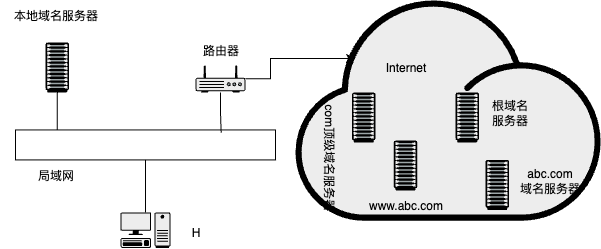
\includegraphics[scale=0.6]{计网图1.png}
    \end{figure}
    A.10ms,\ 40ms\qquad B.10ms,\ 50ms\qquad C.20ms,\ 40ms\qquad D.20ms,\ 50ms

    \item 文件传输协议(FTP)的一个主要特征是() \\
    A.允许客户指明文件的类型但不允许指明文件的格式 \\
    B.不允许客户指明文件的类型但运行指明文件的格式 \\
    C.允许客户指明文件的类型与格式 \\
    D.不允许客户指明文件的类型与格式 

    \item 匿名FTP访问通常使用()作为用户名 \\
    A.guest\qquad B.E-mail地址\qquad C.anonymous\qquad D.主机id

    \item 下列关于POP3协议的说法,()是错误的 \\
    A.由客户端而非服务器选择接收后是否将邮件保存在服务器上
    B.登录到服务器后,发送的密码是加密的 \\
    C.协议是基于ASCII码的,不能发送二进制数据 \\
    D.一个账号在服务器上只能有一个邮件接收目录 

    \item 下面的()协议中,客户机与服务器之间采用面向无连接的协议进行通信. \\
    A.FTP\qquad B.SMTP\qquad C.DNS\qquad D.http

    \item 仅需Web服务器对HTTP报文进行响应,但不需要返回请求对象时,HTTP请求报文应该使用的方法是() \\
    A.GET\qquad B.PUT\qquad C.POST\qquad D.HEAD

    \item 下列关于Cookie的说法中,错误的是() \\
    A.Cookie存储在服务器端\qquad B.Cookie是服务器产生的\\
    C.Cookie会威胁客户的隐私\qquad D.Cookie的作用是跟踪用户的访问和状态

\end{enumerate}
\subsection{25竟成}

\begin{enumerate}
    \item 传输层上使用套接字的主要优点是(\qquad) 
    \begin{choices}[1]
        \task 使客户机与服务器的通信更加快捷 
        \task 能够完成点对点通信
        \task 降低服务器请求失败的可能性
        \task 当请求服务器时可以使用面向连接的协议
    \end{choices}

    \item 以下协议与其他熟知端口号的对应关系正确的是(\qquad)
    \begin{choices}
        \task DNS:80
        \task HTTP:69
        \task SMTP:20
        \task TELNET:23
    \end{choices}

    \item TCP报文中目的端口号的作用是(\qquad)
    \begin{choices}
        \task 指定服务器
        \task 指定请求的服务
        \task 指定传输方式
        \task 指定报文长度
    \end{choices}

    \item 长度为2000B的应用层数据依次封装成TCP报文段,IP数据报和以太网的帧后传送出去(不考虑前导码以及以太网帧拆分情况),
    则数据的最高传输效率为(\qquad)
    
    \item 以下说法错误的是(\qquad)
    \begin{choices}[1]
        \task UDP是无连接的,TCP是面向连接的
        \task UDP比IP多了复用分用和数据差错检测的功能
        \task 一个进程使用UDP协议,另一个进程使用TCP协议,它们可以同时使用同一端口号,
        当从网络层获取数据时,可以根据协议类型实现分用
        \task HTTP协议通信过程中,客户端使和服务端都使用80号端口
    \end{choices}

    \item 下列网络应用中,(\qquad)不适合使用UDP协议. 
    \begin{choices}[2]
        \task 客户-服务器领域
        \task 远程调用
        \task 实时多媒体应用
        \task 远程登录
    \end{choices}

    \item 以下关于UDP校验和的描述中,错误的是(\qquad)
    \begin{choices}[1]
        \task 计算校验和的时候,需要4字节对齐,若数据部分不足,需用0比特填充
        \task 校验和检查UDP的首部和数据部分
        \task 检验处UDP数据报错误的时,可以丢弃或报告上层
        \task UDP校验和能检验UDP数据报外,还能检验IP数据报的源IP地址和目的IP地址.
    \end{choices}

    \item TCP是面向字节流的传输协议,关于TCP报文段长度的表达,正确的是(\qquad)
    \begin{choices}[1]
        \task TPC报文段长度根据每次应用进程需要传输的数据块长度决定
        \task TCP报文段长度根据路径上能够传送的最大数据块长度决定
        \task TCP报文段长度根据接收方的接受能力和网络状态决定
        \task TCP报文段长度确定后,在本应用进程通信过程中保持不变
    \end{choices}

    \item 一个TCP连接的数据传输阶段,如果发送端的发送窗口由2000变成3000,意味着发送端可以发送(\qquad)
    \begin{choices}[1]
        \task 在接受到一个确认前可以发送3000个TCP报文段
        \task 在收到一个确认之前可以发送1000B
        \task 在收到一个确认之前可以发送3000B
        \task 在接受到一个确认前可以发送1000个TCP报文段
    \end{choices}

    判断正误:
    \begin{enumerate}
        \item [(1)] 网络拥塞窗口是发送端根据网络的拥塞程度和接收端的接受能力而设定的. 
        \item [(2)] 将流量控制用于TCP数据传输的原因是为了防止输入数据耗尽接收方资源
    \end{enumerate}

    \item 主机A和主机B刚建立TCP连接时候,约定最大的报文段为2KB,假设主机B的接受窗口为20KB,且保证及时
    清空缓存,拥塞门限值为16KB,RTT=10ms,在不发送拥塞的情况下.则经过(\qquad)ms主机A的发送窗口第一次为20KB.

    \item 主机甲和主机乙新建了一个TCP连接,甲的初始拥塞门限值为32KB,甲向乙始终以MSS=1KB的大小段发送数据.乙
    未该连接分配16KB接受缓存,并对每一个数据段进行确认,忽略其余延迟.若乙收到数据后全部收入缓存,不被取走,则甲从连接
    成功时刻起,未发生超时的情况下,经过4个RTT后,甲的发送窗口大小为(\qquad)
    \begin{choices}
        \task 1KB
        \task 8KB
        \task 16KB
        \task 32KB
    \end{choices}
\end{enumerate}

\subsection{强化1000题}

\begin{enumerate}
    \item 考虑一条点对点链路, 其带宽为$100Mbps$,单向传播时延为10ms,若要使得该链路在数据连续发送时可以得到
    充分利用,则发送方至少需要准备(\qquad bit)才能在第一个比特到达接收端时,发送方仍在发送数据.

    \item 在分层网络体系结构中,从第N+1层传递到第N层,以请求第N层完成某种功能的数据单元称为(\qquad)
    \item 以下说法中,关于计算机网络体系结构中N层PDU和N+1层SDU的关系正确的是(\qquad)(多选)
    \begin{choices}[1]
        \task 一个N+1层的SDU可以封装在一个N层的PDU中
        \task 多个N+1层的SDU可以封装在一个N层的PDU中
        \task 一个N+1层的SDU可以分片封装在多个N层的PDU中
    \end{choices}
    \item 在OSI参考模型中,当相邻高层的实体把(\qquad)传到低层实体后,被底层实体视为(\qquad) 
    \item 在网络体系结构中,各层的PDU由SDU和PCI组成,OSI参考模型自下而上的第一层,第二层,第三层的SDU分别是(\qquad),(\qquad),(\qquad)
    \item 下列关于OSI/RM的描述中错误的是(\qquad)(多选)
    \begin{choices}[1]
        \task 10Base-T中"T"的含义,属于物理层的范畴
        \task 物理地址,硬件地址和MAC地址,都属于数据链路层的范畴
        \task 网络层不涉及拥塞控制功能
        \task 运输层为上层提供端到端的服务
        \task 应用层使用其下层提供的服务,在本层协议的控制下实现网络应用
    \end{choices}
    \item 调制解调技术主要使用在(\qquad)通信方式中
    \item 采用FSK进行数字数据调制时,是通过改变载波信号的(\qquad)参数来表示不同的数字比特
    \item 下列选项中包含同步信息的编码是(\qquad)(多选)
    \begin{choices}
        \task 归零编码
        \task 非归零编码
        \task 曼彻斯特编码
        \task 差分曼彻斯特编码
    \end{choices}
    \item 下列关于数据交换方式叙述正确的是(\qquad)
    \begin{choices}[1]
        \task 报文交换传输延迟最大但服务可靠
        \task 电路交换传播延迟最下且服务最可靠
        \task 分组交换传播延迟最小且服务最不可靠
        \task 分组交换总延迟最大但服务最可靠
    \end{choices}

    \item 在10Mbps的以太网标准中,规定最小帧长为(\qquad)如果一个站点发送了一个小于其的帧,集线器会如何处理这个帧(\qquad)? 
    \begin{choices}[1]
        \task 丢弃该帧,因为它太短了
        \task 自动填充至最短帧的长度
        \task 正常放大并转发该帧
        \task 向发送端发送一个错误信号
    \end{choices}

    \item 在数据帧中,当所传送的数据中出现控制字符时,就必须采取适合的措施,使接收方不至于将数据误认为是控制信息.
    这样才能保证数据链路层传输是(\qquad)

    \item 一个采用奇校验进行编码的系统,如果接收端收到的8位码字为\underline{10110010},那么接收端会判定(\qquad)

    \item 某数据块\underline{1010110}计划采用偶校验方式发送,校验码附加在数据块的末尾.则实际发送的比特序列应该为(\qquad)
    \item 关于奇偶校验,下列说法中均正确的是(\qquad)
    \begin{choices}[1]
        \task 水平奇偶校验码是在数据块的每一列之后附加校验位
        \task 单独使用水平奇偶校验或者垂直奇偶校验,均可以检测出数据块内任意两个比特同时发生的错误
        \task 二维奇偶校验结合律水平校验和垂直校验,不仅能检测出所有单个,两个和三个比特的错误,还能确定并纠正单个比特的错误
        \task 垂直奇偶校验产生的方块校验字符的主要目的是压缩数据一提高传输效率,其检错能力较弱
    \end{choices}

    \item 下列位串,可以作为生成多项式系数序列是(\qquad)
    \begin{choices}
        \task 1101 \task 0110 \task 1100 \task 0101
    \end{choices}

    \item 如果一个编码方案被设计用来检测e位错误,纠正t位错误,同时检测e位错误并纠正t位错误,其最小海明距离d分别不小于(\qquad)
    \item 关于停止-等待协议,下列说法错误的是(\qquad)
    \begin{choices}[1]
        \task 对于停止-等待协议,重传的请求是发送方自动进行的
        \task 超时重传时间RTO一般设置为略大于收发双方的平均往返时间
        \task 数据链路层一般不会出现确认分组迟到的情况,因此数据链路层实现停止-等待协议可以不用给确认分组编号
        \task 停止-等待协议的信道利用率一定比其他接收窗口不为1的协议低
    \end{choices}

    \item 在一个采用GBN协议的系统中,若用于帧编号的比特数为4,发送方已经发送了发送窗口可以发送的最大数量的帧,且刚收到
    ACK12,则发送方还能继续发送(\qquad)个数据帧

    \item 数据链路层采用GBN协议,数据传输速率为1Mbps,单向传播时延为200ms,数据帧长度范围是$\left[500,1500\right]$字节,确认帧
    长度总与数据帧相同.为使信道利用率达到最高,帧序号的比特数至少为(\qquad)

    \item 采用SR协议,发送窗口与接受窗口均为4,主机甲向主机乙发送数据.初始时,甲的发送窗口是[0,1,2,3],甲发送了0,1号帧,随后收到ACK1.
    然后甲发送了2,3帧,此时,甲的窗口内待确定的帧的集合是(\qquad)

    \item 下列关于时分复用(TDM)的说法正确的是(\qquad)
    \begin{choices}[1]
        \task 共享信道的总带宽必须精确划分并分配给每个用户,且用户带宽之和等于信道总带宽
        \task 共享信道的数据传输速率必须至少等于所有用户数据传输速率的总和
        \task TDM技术采用介质的位速率可以小于单个信号的位速率
        \task 每个用户在分配到的时间片内发送数据前,仍然需要通过载波监听来避免与其他用户发生冲突
    \end{choices}

    \item 在设计信道复用系统时,为防止相邻用户信号间的潜在串扰,通常需要在分配的资源之间设置一定的保护间隔.
    (\qquad)信道复用技术因为其信号隔离机制的特性,对这类因保护间隔而引入的频谱或时间效率损失最为敏感,
    且该间隔是其设计中不可或缺的物理隔离手段?

    \item 站点D的码片序列为\{1,1,-1,-1\},若信道上接收到的序列是\{2,2,-2,2,0,0,0,-4,-2,2,2,2\},则站点D发送的数据是(\qquad)

    \item 若在CDMA系统中,A 要通过基站跟 B 通信,A、B 的码片序列分别是 
    (1,1,1,1)、(1,-1,1,-1),如果 A 想给 B 发送的一些数据中含一个比特信息“0”,
    那么 A 发出的序列中比特“0”对应的序列是(\qquad),B 收到的序列该比特 0 对应的序列是(\qquad)

    \item 关于纯ALOHA协议与时隙ALOHA协议的比较,下列说法错误的是( ).
    \begin{choices}[1]
    \task 两者都属于随机访问协议
    \task 时隙ALOHA协议比纯ALOHA协议具有更高的最大信道利用率
    \task 纯ALOHA协议不需要全局时间同步,而时隙ALOHA协议需要
    \task 纯ALOHA协议发生冲突后不进行重传,而时隙ALOHA协议会重传
    \end{choices}

    \item  在ALOHA类型的协议中,发送方判断是否发生碰撞的主要依据是()
    \begin{choices}[1]
    \task 接收到来自其他站点的NACK信号
    \task 监听到信道上出现干扰信号
    \task 在预设的超时时间内未收到接收方的确认(ACK)
    \task 物理层报告的载波丢失
    \end{choices}

    \item 在CSMA(载波侦听多路访问)协议中,与1-坚持CSMA相比,非坚持CSMA的主要优点是().
    \begin{choices}[1]
    \task 减少了信道空闲时的等待时间
    \task 减少了多个站点在信道变空闲后立即发送而导致的冲突概率
    \task 信道利用率总是更高
    \task 实现更简单
    \end{choices}

    \item  关于p-坚持CSMA协议的特点,下列说法中错误的是().
    \begin{choices}[1]
    \task 该协议旨在综合1-坚持CSMA的低延迟特性和非坚持CSMA的低冲突特性.
    \task 参数p的选择对协议性能有显著影响,p值越小,站点发送前等待的平均时隙数越多.
    \task 当监听到信道空闲时,站点以概率p发送数据;若未发送,则以概率(1-p)在当前时隙继续监听.
    \task 若参数p设置为1,则p-坚持CSMA协议的行为特性基本等同于1-坚持CSMA协议.
    \end{choices}

    \item 某局域网采用CSMA/CD协议,主机A和主机B的距离为1km,传播速率为$2*10^5km/s$.t=0时,A发送
    了数据帧,在A数据发送完毕前,B也发送了数据帧,A、B检测到碰撞的时间相差3us,则B发送数据的时
    间和A,B发送的数据发生碰撞的时间为(\qquad)

    \item 在CSMA/CD的局域网中,假设所有帧发送需要的时间是To,端到端单程的时延为t,那么该信道的最大利用率为(\qquad)

    \item 关于NAV,下列说法错误的是? (\qquad)
    \begin{choices}[1]
    \task NAV是一种虚拟载波侦听机制,用于指示介质被占用的预期时间.
    \task 站点会将其NAV设置为RTS/CTS帧中声明的持续时间值.
    \task 当一个站点的NAV值大于0时,即使物理载波侦听显示介质空闲,它也必须推迟发送.
    \task 一个站点自身的NAV计时器会随时间递减,当NAV为0时,如果物理信道也空闲,则可以尝试接入信道.
    \end{choices}

    \item 在采用CSMA/CA的802.11无线局域网中,若采用RTS/CTS机制,已知DIFS为120us,SIFS为28us,RTS帧、CTS、
    ACK帧的发送时延分别为3us、2us、2us,数据帧的发送时延为296us,信号传播时延忽略不计.
    主机A通过RTS/CTS机制向AP发送一个数据帧.若邻近主机A的站点C(非AP)能够正确接收到A发送的RTS帧,
    但由于位置关系听不到AP发送的CTS帧,则站点C在其NAV中设置的持续时间应为(\qquad)

    \item 局域网的协议一般不包括(\qquad)的内容.
    \item 上层协议交给数据链路层的数据长度为32B,则数据链路层会(\qquad)
    \item 以太网V2帧格式没有显式的结束定界符,它是如何确定帧的结束的? (\qquad)
    \begin{choices}[1]
    \task 通过帧首部的长度字段
    \task 通过检测到信道上不再有信号(载波消失)
    \task 通过物理层编码违例
    \task 通过校验和字段的特定值
    \end{choices}

    \item 关于千兆以太网在半双工模式下采用的载波延伸和新的争用期,下列说法中正确的是(\qquad)
    \begin{choices}[1]
    \task 载波延伸是通过在MAC帧的数据字段内部填充0比特,使其实际长度达到512字节.
    \task 新的争用期被定义为发送64字节数据所需的时间,以保持与传统以太网的兼容性.
    \task 若MAC帧的长度(包括首部和FCS)已达到或超过512字节,则发送该帧时不再需要进行载波延伸.
    \task 载波延伸所添加的特殊符号会被接收方的MAC子层作为有效数据处理,并向网络层提交.
    \end{choices}

    \item 关于半双工千兆以太网中分组突发机制,下列说法中正确的是(\qquad)
    \begin{choices}[1]
    \task 允许一个站点在检测到信道空闲后,可以无视CSMA/CD协议,连续发送任意数量的帧.
    \task 通过将多个短帧合并成一个超长帧进行发送,减少了头的开销.
    \task 对于需要发送多个连续短帧的站点,在成功获得一次介质访问权后,可以持续发送一段帧序列,从而减少了为每个短帧重新竞争信道所带来的开销和延迟.
    \task 使得在发生碰撞后,站点能够以更快的速率重传所有在突发期间未能成功发送的帧.
    \end{choices}

    \item 关于IEEE802.11无线局域网中的BSS,下列说法中错误的是(\qquad).
    \begin{choices}[1]
    \task 在基础设施模式BSS中,所有无线站点之间的通信都必须经过接入点(AP)中转.
    \task 无固定设施的无线局域网中的BSS,允许无线站点之间直接通信,无需AP的存在,也称为Ad Hoc网络.
    \task 每个BSS都由一个唯一的SSID(服务集标识符)来全局唯一地命名和区分,SSID通常就是AP的MAC地址.
    \task 一个BSS内的所有站点通常共享相同的物理层特性,例如在相同的信道上工作.
    \end{choices}

    \item 关于IEEE802.11无线局域网的SSID,下列说法中错误的是(\qquad)
    \begin{choices}[1]
    \task SSID是一个长度可变的字符串,最多可以包含32个字符,用于标识一个无线网络.
    \task 接入点(AP)通常会在信标帧中广播其SSID,以便客户端发现.
    \task 为了实现无缝漫游,在一个扩展服务集(ESS)内的所有AP必须配置不同的SSID.
    \task 用户在连接无线网络时,通常需要从可用网络列表中选择一个SSID.
    \end{choices}

    \item 在一个ESS中,接入点AP1(MAC地址为00-12-34-AA-BB-CC)和接入点AP2(MAC地址为00-12-34-DD-EE-FF)
    通过无线链路互连.现有一个数据帧,其原始发送站点为STA1(MAC地址为00-DE-AD-BE-EF-01),
    最终接收站点为STA2(MAC地址为00-DE-AD-CA-FE-02).该数据帧由AP1经无线链路转发给AP2.
    在此无线转发过程中,AP1发送给AP2的这个IEEE802.11数据帧F,其帧头中的地址1、地址2、地址3和地址4字段的内容
    分别是(\qquad)

    \item 下列关于令牌环网络的描述,错误的是( )
    \begin{choices}[1]
    \task 每个站点都可以持有令牌一段固定的时间,没有数据要发的站点收到令牌后会立刻传递下去.
    \task 令牌环网的主要功能是提供可靠的数据冲突检测与解决机制.
    \task 使用令牌在网络中轮流传递,同一时刻,环上只有一个数据在传输.
    \task 令牌环网通常应用于高速局域网(LAN)环境和无线传感网络.
    \end{choices}

    \item 下列关于802.1Q帧的说法中,错误的是( )
    \begin{choices}[1]
    \task 与802.3以太网帧不同,802.1Q帧的最大帧长度为1522字节.
    \task 当802.1Q帧经过Trunk接口转发出去时,Trunk接口将会去除802.1Q帧的标签.
    \task 当且仅当Access接口的PVID值与帧的PVID相同时,Access接口才会转发该帧.
    \task 802.1Q帧VID取值范围为0到4095,其中0和4095保留不用.
    \end{choices}


    \item 下列关于广域网和互联网(Internet)关系的描述,正确的是( )
    \begin{choices}[1]
    \task 广域网就是互联网
    \task 互联网是世界上最大的局域网
    \task 互联网可以由许多广域网、局域网通过路由器互连而成
    \task 广域网必须通过互联网才能实现远程通信
    \end{choices}


    \item 关于PPP协议提供的服务特性,下列说法正确的是( )
    \begin{choices}[1]
    \task PPP提供可靠的、面向连接的数据传输服务
    \task PPP通过序号和确认机制保证数据按序到达
    \task PPP提供差错检测功能,能丢弃有差错的帧
    \task PPP协议内置了复杂的流量控制机制
    \end{choices}


    \item 在使用PPP协议的异步线路上,若要发送的数据字节为0x7D(PPP的转义字符),则实际在线路上传输的字节序列是( )
    \item IPCP协议专门负责在PPP链路上建立、配置和终止IP协议的运行,该协议属于下列PPP协议中
    哪个组成部分的功能?(\qquad)
    \begin{choices}[1]
    \task 物理层接口定义
    \task 链路控制协议(LCP)
    \task 网络控制协议(NCP)
    \task 身份验证协议        
    \end{choices}

    \item  当PPP链路的一端检测到其物理层不再可用时(例如,调制解调器检测到载波丢失).PPP链路状态会转换到( )
    \begin{choices}[1]
    \task 链路终止状态
    \task 网络层协议状态
    \task 链路死亡状态
    \task 链路建立状态,尝试重新建立
    \end{choices}

    \item 下列关于PPP帧的说法错误的是( )
    \begin{choices}[1]
    \task PPP帧的地址(Address)字段固定为0xFF.这是因为该帧是一个广播帧,发送给链路上所有可能的接收者.
    \task 与MAC帧不同,PPP帧的最短帧长是16字节.
    \task 为确保帧定界符的唯一性,PPP协议在传输信息字段时会采用字节填充或比特填充技术以实现透明传输.
    \task PPP协议支持在同步和异步链路上运行,并能封装多种网络层协议.
    \end{choices}

    \item 下列关于以太网交换机和路由器的比较,描述错误的是?
    \begin{choices}[1]
    \task 交换机通常根据MAC地址转发数据帧,路由器通常根据IP地址转发IP数据包.
    \task 交换机可以隔离冲突域但不能隔离广播域(默认情况),路由器既可以隔离冲突域也可以隔离广播域.
    \task 交换机不修改通过它的数据帧的源MAC和目的MAC地址(透明传输),路由器在转发IP数据包时通常会修改源MAC和目的MAC地址.
    \task 交换机和路由器都使用最长匹配原则进行转发决策.
    \end{choices}

    \item 关于以太网交换机的直通交换方式,下列说法中错误的是?
    \begin{choices}[1]
    \task 直通交换方式的转发延迟通常小于存储转发方式
    \task 直通交换方式在转发决策时仅需检查帧的目的MAC地址.
    \task 直通交换方式可能会将一些包含差错的帧转发出去.
    \task 直通交换方式依赖其快速转发能力,能够自动协商并匹配输入与输出端口间可能存在的速率差异.
    \end{choices}

    \item 下列关于虚电路网络的描述中,错误的是(\qquad)
    \begin{choices}[1]
    \task 在数据传输阶段,所有分组都沿着建立虚电路时确定的路径进行传输。
    \task 需要为一条虚电路预留带宽等资源,以保证可靠传输。
    \task 网络中的节点需要为每条经过它的虚电路维护一条记录。
    \task 每个分组的首部不需要包含完整的源地址和目的地址。
    \end{choices}

    \item 若网络层提供的是虚电路服务,那么当一条虚电路上的某个中间节点发生故障时,最直接的后果是(\qquad)
    \begin{choices}[1]
    \task 后续分组会自动选择其他路径绕行。
    \task 只有当前正在该节点处理的分组会丢失。
    \task 该虚电路被破坏,其上的所有通信都会中断。
    \task 源主机会立即收到一个ICMP差错报文。
    \end{choices}

    \item 在SDN体系结构中,SDN控制器主要负责以下哪项功能?
    \begin{choices}[1]
    \task 根据流表规则直接转发用户数据包
    \task 执行网络应用程序定义的业务逻辑
    \task 维护全网的拓扑视图并计算路由、生成流表下发给交换机
    \task 物理层信号的编码与解码
    \end{choices}

    \item 主机A向主机B发送一个IP数据报,其首部中DF位置为1。该数据报在到达路由器R1时,R1发现其长度超过了下一跳链路的MTU。此时,R1应如何处理?
    \begin{choices}[1]
    \task 丢弃该数据报,并向主机A发送ICMP“超时”差错报文。
    \task 对数据报进行分片,保证每个分片的长度为8的倍数且小于下一跳MTU,然后进行转发。
    \task 丢弃该数据报,并向主机A发送ICMP“目的不可达”差错报文。
    \task 丢弃该数据报,但不发送任何ICMP差错报文以节省网络资源。
    \end{choices}

    \item 下列关于IP地址的说法中,错误的是(\qquad)
    \begin{choices}[1]
    \task IP地址不能反映任何有关主机位置的物理信息
    \task 一个主机同时连接在多个网络上时,该主机只能拥有一个自己的IP地址
    \task 由转发器或网桥连接起来的若干个局域网仍为一个网络
    \task IP地址可用来指明一个网络的地址
    \end{choices}

    \item NAT路由器采用端口映射技术。假设内网中的主机H1(192.168.0.33)和H2(192.168.0.44)同时访问外部Web服务器,且它们使用的源端口号恰好相同(均为1025)。NAT路由器的公网IP为202.10.10.1。下列关于经过NAT转换后发出的两个IP分组的描述,正确的是(\qquad)
    \begin{choices}[1]
    \task 两个分组的源IP地址不同,源端口号相同
    \task 两个分组的源IP地址相同,源端口号也相同
    \task 两个分组的源IP地址相同,但源端口号必不相同
    \task 路由器将无法处理第二个分组,因为源端口号冲突
    \end{choices}

    \item 下列IP地址中,只能作为IP分组的目的IP地址但不能作为源IP地址的是(\qquad)
    \begin{choices}[2]
    \task 0.0.0.0
    \task 127.0.0.1
    \task 20.10.10.3
    \task 223.255.255.255
    \end{choices}

    \item 下列IP地址中,不能作为IP数据报源地址,只能作为目的地址的是(\qquad)
    \begin{choices}[2]
    \task 10.1.1.1
    \task 172.16.255.255
    \task 224.0.0.5
    \task 127.0.0.1
    \end{choices}

    \item 现将一个IP网络划分成4个子网,若其中一个子网是172.16.1.128/26,则下列网络中,不可能是另外三个子网之一的是(\qquad)
    \begin{choices}[2]
    \task 172.16.1.0/25
    \task 172.16.1.64/26
    \task 172.16.1.96/27
    \task 172.16.1.224/27
    \end{choices}

    \item IP地址为128.5.3.4、子网掩码为255.255.255.0的主机所在的网络,最多可以划分为M个子网,每个子网内最多可以有N台主机,M和N分别为(\qquad)
    \begin{choices}
    \task 254,254
    \task 62, 2
    \task 62, 254
    \task 126, 2
    \end{choices}

    \item 某网络的IP地址空间为192.168.5.0/24,采用变长子网掩码(VLSM)来划分子网以满足不同部门的需求:部门A需要50台主机,部门B需要20台主机,部门C需要10台主机。如果按照所需IP地址数从大到小的顺序分配地址空间,则分配给部门B的子网的网络地址可能是(\qquad)
    \begin{choices}[2]
    \task 192.168.5.0
    \task 192.168.5.64
    \task 192.168.5.96
    \task 192.168.5.128
    \end{choices}

    \item 主机H1的IP地址为192.168.1.10/24,其配置的默认网关为192.168.1.1。现主机H1希望向另一台主机H2(IP地址为192.168.2.20/24)发送IP数据包。假设主机H1的ARP缓存为空。在此通信场景下,主机H1首先会发送ARP请求的目标IP地址是(\qquad)
    \begin{choices}[2]
    \task 192.168.1.1
    \task 192.168.2.20
    \task 192.168.1.255
    \task 255.255.255.255
    \end{choices}

    \item 在一个局域网中,主机A发送一个ARP请求以查询主机B的MAC地址。当该ARP请求帧到达交换机时,交换机通常会如何处理?
    \begin{choices}[1]
    \task 仅将该帧转发给连接主机B的那个端口
    \task 丢弃该帧
    \task 向除接收端口外的所有其他端口转发该帧
    \task 查询自身的ARP缓存表,若有对应条目则直接代答
    \end{choices}

    \item 下列关于ARP协议的说法中,正确的是(\qquad)
    \begin{choices}[1]
    \task ARP请求和ARP响应报文均封装在IP数据报中,由IP协议负责其传输
    \task 为防止ARP欺骗,ARP协议自身设计了严格的安全验证机制来确认应答的合法性
    \task 目标主机收到ARP请求报文后,仅发送ARP响应报文而不做其他操作
    \task ARP协议除了ARP请求报文和响应报文外,还有其他类型的报文
    \end{choices}

    \item 以下选项中不属于ICMP报文的是(\qquad)
    \begin{choices}[2]
    \task 地址掩码请求/应答报文
    \task 源站抑制报文
    \task 流量调整报文
    \task 回送请求/应答报文
    \end{choices}

    \item 当一个长度为3000字节的TCP报文段需要从源主机发送到目的主机时,假设源主机和目的主机之间的路径上的MTU为1400字节,假设在网络传输过程中不发生丢包、重传等问题,下面说法正确的是(\qquad)
    \begin{choices}[1]
    \task 为了将TCP报文段正确传输到目的主机,源主机需要分为3个IP数据报,且IP数据报的总长度分别为1400,1400和260
    \task 第3个分片的MF标志位为0,DF标志位为1
    \task 如果第1个分片的标识位是12345,则第2个分片的标识位是12346,第3个分片的标识位是12347
    \task 在收到最后一个IP数据报之后,目的主机需要查看每个数据报的MF标志位,将数据报的TCP数据字段按照顺序依次组装成一个完整的TCP报文段
    \end{choices}

    \item 下列关于IPv4和IPv6的叙述中,正确的是(\qquad)
    \begin{choices}[1]
    \task 采用双协议栈进行IPv4数据报和IPv6数据报之间的转换,会导致数据报部分首部信息丢失
    \task IPv6用有效载荷长度字段记录自己除了基本首部和扩展首部外数据载荷部分的长度
    \task IPv6缺少协议字段,因此无法指明何种协议数据单元PDU
    \task IPv6可以解决IPv4地址耗尽的问题
    \end{choices}

    \item 一个IPv6的简化写法为8::D0:123:CDEF:89A,那么它的完整地址应该是()
    \begin{choices}[1]
    \task 8000:0000:0000:0000:00D0:1230:CDEF:89A0
    \task 0008:0000:0000:0000:00D0:0123:CDEF:89A0
    \task 8000:0000:0000:0000:D000:1230:CDEF:89A0
    \task 0008:0000:0000:0000:00D0:0123:CDEF:089A
    \end{choices}

    \item 下列关于路由信息协议RIP的说法中正确的是(\qquad)
    \begin{choices}[1]
    \task RIP协议的核心功能是路由选择,是网络层协议,被网络层IP协议封装。
    \task 当存在多条到达同一目的网络的路由时,路由器只会保存其中最新的,以保证路由信息的可靠性。
    \task 相较于OSPF协议,RIP协议实现简单,路由器开销小,更适合路由器数目较多的网络。
    \task 当网络拓扑发生变化时,路由器要及时向相邻路由器通告拓扑变化后的路由信息以加快RIP的收敛速度。
    \end{choices}

    \item 一个采用RIP协议的路由网络中,路由器R1的当前路由表有一条到达网络N的路由,其下一跳为R3,跳数为8。此时,R1又收到了来自邻居路由器R2的更新报文,其中包含路由信息<N,7>。R1将如何更新路由表?
    \begin{choices}[1]
    \task 维持原路由不变
    \task 到网络N的路由,下一跳改为R2,跳数为7
    \task 到网络N的路由,下一跳改为R2,跳数为8
    \task 新增一条到网络N的备用路由,下一跳为R2,跳数为8
    \end{choices}

    \item 在OSPF的多区域结构中,关于骨干区域的描述,正确的是(\qquad)
    \begin{choices}[1]
    \task 骨干区域是唯一可以与外部自治系统相连的区域。
    \task 骨干区域内的路由器不能成为区域边界路由器(ABR)。
    \task 所有非骨干区域都必须与骨干区域直接相连。
    \task 骨干区域只负责传递路由信息,不承载用户数据流量。
    \end{choices}

    \item 在两个自治系统的边界路由器R1和R2之间成功建立了BGP连接。在运行过程中,R1从R2收到了一个UPDATE报文,但在解析时发现该报文中缺少一个BGP协议定义的某个属性。根据BGP协议的规定,R1此时应当发送下列哪种报文来响应这一差错情况?
    \begin{choices}[1]
    \task OPEN
    \task KEEPALIVE
    \task UPDATE
    \task NOTIFICATION
    \end{choices}

    \item 一个IP组播组的成员是(\qquad)
    \begin{choices}[1]
    \task 物理上位于同一地理区域的一组主机。
    \task 逻辑上属于同一个IP子网的一组主机。
    \task 一组希望接收发往同一个特定组播地址的数据的主机集合,其成员是动态变化的。
    \task 一组由网络管理员预先配置好的、固定不变的主机。
    \end{choices}

    \item 网际组管理协议(IGMP)运行于()之间。
    \begin{choices}[1]
    \task 组播源主机和组播目的主机。
    \task 两台组播路由器。
    \task 主机和它的本地组播路由器。
    \task 应用层进程和运输层协议。
    \end{choices}

    \item 以下有关IP多播的相关描述中,错误的是(\qquad)
    \begin{choices}[1]
    \task IP多播需要使用网际组管理协议IGMP和普通路由选择协议。
    \task IP多播分为两种:一种是只在本地局域网上进行硬件多播,另一种则是在因特网的范围进行多播。
    \task IP多播使用D类IP地址。
    \task IP多播地址只能用于目的地址,而不能用于源地址。
    \end{choices}

    \item 当一个局域网内的多台主机都加入了同一个IP组播组时,如果本地路由器发送了一个IGMP普通查询报文,将会发生什么?
    \begin{choices}[1]
    \task 所有加入该组的主机都会立即回复一个成员报告报文。
    \task 只有一台主机需要回复成员报告报文,其他主机侦听到后会抑制自己的回复。
    \task 只有新加入的主机会回复。
    \task 只有该组播组选举出的代表主机会回复。
    \end{choices}

    \item IGMP成员查询报文被封装在IP多播数据报中,IP多播数据报的目的地址和生存时间TTL分别为(\qquad)
    \begin{choices}[2]
    \task 224.0.0.1, 1
    \task 224.0.0.1, 255
    \task 224.0.0.2, 1
    \task 224.0.0.2, 255
    \end{choices}

    \item 在以下有关IP路由器的相关描述中,正确的是(\qquad)
    \begin{choices}[1]
    \task IP路由器不涉及拥塞控制功能。
    \task 给路由器的接口配置好IP地址和地址掩码后,路由器会自动得出该接口的直连网络地址。
    \task 使用1.1.1.1/32表示默认路由。
    \task 使用0.0.0.0/0表示特定主机路由。
    \end{choices}

    \item 网络互连时,在由路由器进行互连的多个局域网的结构中,要求每个局域网的(\qquad)
    \begin{choices}[1]
    \task 物理层协议可以不同,而数据链路层及数据链路层以上的高层协议必须相同。
    \task 物理层、数据链路层协议可以不同,而数据链路层以上的高层协议必须相同。
    \task 物理层、数据链路层、网络层协议可以不同,而网络层以上的高层协议必须相同。
    \task 物理层、数据链路层、网络层及高层协议都可以不同。
    \end{choices}
\end{enumerate}
\section{综合题}

\newpage

\section{选择题答案}
\subsection{25-王道-答案}
\begin{enumerate}
    \item 
\end{enumerate}
\subsection{25-竟成-答案}
\begin{enumerate}
    \item B;
    \item D; 计算机网络显然将各个独立的计算机相互连接成一个分布式系统
    \item D; 操作系统是一个比较宽泛的概念
    \item B; 广域网使用的是PPP(点对点协议),局域网使用的是以太网协议(IEEE 802系列协议)
    \item C; 典型拓扑的常见应用有 {\color{red} 现代以太网LAN:星型, 园区/校园:树型, 城域网:环型, 广域网:网状}
    \item D; 注意TCP/IP体系结构和OSI体系结构的区别! 在OSI体系结构中数据链路层在不可靠的物理层介质上提供可靠的传输,
    其功能包括物理寻址,成帧,流量控制,差错检验,数据重发等功能,
    \item D; {\color{red} 重要区别,TCP/IP中运输层提供面向连接(TCP)和无连接(UDP)的连接方式,而ISO/OSI体系结构中
    网络层提供两种连接方式,而运输层仅提供面向连接的通信}
    \item 
    \item 选A; 套接字(socket)本质是IP地址+端口号,是传输层的T-SAP(传输服务访问点). 传输层并不提供{\color{red}点到点,而是提供端到端(进程到进程)间的通信}
    需要注意并非TCP专用套接字,UDP也使用. 
    \item 选D; 应用层协议端口号与对应传输层协议需要多记
    \item 选B; 服务器由IP地址决定,传输方式由所使用的协议决定,报文长度由报文首部决定
    \item 97.19\%; 需要熟练记忆各协议首部的长度以及关键参数 
    \item D; HTTP协议的客户端端口为动态分配,服务器为熟知端口80
    \item D; UDP的特点是效率高,开销小,延迟低;但不保证数据准确.通常不用于需要持久性连接的应用.
    \item A; 计算校验和需要{\color{red} 2字节对齐而非4字节对齐} 
    \item C;
    \item C; 这题并不严谨,主要是记录TCP是以字节为单位控制窗口而非TCP端 \\
    判断正误: 错, 网络拥塞窗口->发送窗口 \\
    判断正误: 对
    \item 50ms; 注意MSS=2KB, 其变化规律应该是4KB->8KB->16KB(到达上限)->18KB-20KB 注意后面每次是加1MSS而非1KB
    \item A; 题设很长注意抓关键点{\color{red} 收入数据后不被取走},发送窗口由接收方窗口大小和拥塞窗口大小的较小值决定.
\end{enumerate}

\subsection{强化1000题-答案}
\begin{enumerate}
    \item 若要使得链路充满bit至少要保证放松数据量大于等于"时延带宽积"即$100Mbp*10ms = 1 * 10^6 bit$
    \item 第D+1层的PDU
    \item ABC 
    \item IDU, SDU 
    \item 帧,分组,报文段
    \begin{remark}[PDU,SDU,IDU三者的关系]
        SDU: Service Data Unit, 服务数据单元. 其是由N+1层往N层传送的原式数据 \\
        IDU: Interface Date Unit, 接口数据单元, 由第N+1层实体通过服务访问点SAP将一个IDU送往第N层(SDU+ICI) \\
        PDU: Protocol Date Unit, 服务数据单元, 第N层对等体间通信所需要交换的数据单元(SDU+对应层报头组成) 
    \end{remark}
    \item AC; 物理层的功能: 规定了一个结点如何连接到传输介质之上(4个特性), 而T代表双绞线是传输介质本身不由物理层管理.\\
    TCP/IP体系下网络层提供无连接尽力而为的服务,但并非完全没有拥塞控制, 不要忘记路由器是有权丢掉分组并返回ICMP报文的
    \item {\color{red} 数字数据}通过调制解调器调制成模拟信号.
    \item 频率; FSK是频移键控的缩写, 使用不同的载波信号来代表不同的数字比特.
    \item ACD 
    \item B 
    \item 64B, C . 集线器(hub)作为物理层设备,他不对数据帧的内容进行检查,短帧的处理由高层负责. 
    \item 透明
    \item 数据传输中发生了奇数个比特的错误
    \item 10101100
    \item C 
    \item A 生成多项式的最高位系数和最低位系数都不能为0
    \item $d\geq e+1, d\geq 2t+1, d\geq t + s + 1$
    \item 
\end{enumerate}

\subsection{26-王道-答案}
\begin{enumerate}
    \item 
\end{enumerate}
\subsection{精选1000题-答案}
\begin{enumerate}
    \item 
\end{enumerate}
\ifx\allfiles\undefined
\end{document}
\fi